\section{Analisi delle differenze sintattiche tra sognatori} \label{sec:analisi-delle-differenze-sintattiche-tra-sognatori}

Come anticipato nel Capitolo~\ref{cap:mondo-dei-sogni}, nel contesto psichiatrico la rappresentazione di testi sui
sogni attraverso grafi si \`e rivelato un'utile strumento a supporto della diagnosi di disturbi come la schizofrenia
o il disturbo bipolare~\cite{mota2014graph}, nonch\'e la possibilit\'a di predire l'insorgenza di patologie in
anticipo rispetto alla diagnosi clinica~\cite{mota2017thought}.
Tali studi evidenziando di come l'attenzione ad aspetti sintattici della descrizione di sogni possano fornire
informazioni significative sullo stato mentale di un individuo. Costruendo grafi in cui i nodi corrispondono a parole
e gli archi ad un loro utilizzo consecutivo, si è rivelato utile valutare aspetti come la presenza di cicli di parole
ricorrenti, la connettivit\'a delle parole e la loro organizzazione in componenti fortemente connesse.

In questa sezione verrà illustrata una possibile metodologia di analisi sintattica dei testi di singoli sogni mediante
grafi multi-livello, applicandola ai sogni di un campione di tre sognatori: Arlie, Emma e Norman.
In particolare, si cercherà di potenziare la modalità di studio proposta dalle ricerche citate, cercando di estenderla
grazie alla visione globale fornita dal grafo multi-livello e focalizzando l'attenzione sugli aspetti che caratterizzano
l'evoluzione dei grafi delle parole nel corso delle contrazioni.

\subsection{Fase di pre-elaborazione}\label{subec:pre-elaborazione-con-NLP}
Prima di applicare la vera e propria analisi attraverso l'impiego dei grafi multi-livello al dataset di sogni, si è
ritenuto necessario effettuare una pre-elaborazione dei testi attraverso gli strumenti tipici dell'elaborazione del
linguaggio naturale.
L'NLP (in inglese \textit{Natural Language Processing}) è di fatti quella disciplina a metà tra intelligenza artificiale
e linguistica che si occupa di individuare i metodi di elaborazione e analisi di dati che si presentano sotto forma di
linguaggio naturale, ovvero di linguaggi usati dell'essere umano. \newline

La pre-elaborazione ha quindi previsto l'applicazione della seguente sequenza di fasi al corpus di sogni originario:
\begin{enumerate}
    \item Pulizia del testo. \newline \noindent
          Questa fase ha incluso la rimozione degli spazi bianchi superflui, la standardizzazione della
          formattazione del testo e la correzione di errori ortografici o di incoerenze. È stata inoltre eseguita la
          rimozione della punteggiatura, snellendo ulteriormente i dati testuali. Tali procedure di pulizia sono
          essenziali per garantire la qualità e la coerenza dei dati in ingresso, migliorando così l'affidabilità
          dell'analisi.
    \item Tokenizzazione. \newline \noindent
          Questa fase ha comportato la suddivisione del testo in parole singole dette \textit{token},
          passaggio fondamentale nell'elaborazione del linguaggio naturale, creando la base per le fasi successive.
    \item Rimozione delle stop words. \newline \noindent
          Le \textit{stop words} sono parole comuni (come ``the'', ``is'', ``at'', ``which'' e ``on'') che tipicamente
          hanno un ruolo significativo nei compiti di NLP, specialmente in quelli legati ad analisi semantiche.
          In questo caso, la loro rimozione può certamente aiutare a concentrare l'analisi sulle parole più ricche di
          contenuto nelle narrazioni dei sogni, riducendo significativamente il rumore nei dati e mettendo in evidenza
          i termini più salienti.
    \item Lemmatizzazione. \newline \noindent
          La lemmatizzazione è un processo che riduce le parole alla loro forma base, chiamata \textit{lemma}.
          Ad esempio, ``running'' verrebbe lemmatizzato in ``run'' e ``better'' in ``good''.
          Questo passaggio aiuta a ridurre le diverse declinazioni delle parole ai loro concetti di base, riducendo
          la dimensionalità dei dati testuali e rivelando, potenzialmente, schemi sottostanti in modo più chiaro.
    \item Costruzione del grafo delle parole. \newline \noindent
          Infine, è stato costruito un grafo diretto basato sulle singole parole all'interno delle sequenze
          di lemmi associate ad ogni sogno. Tali parole, in quanto prese singolarmente rispetto alla sequenza
          di appartenenza, si definiscono \textit{unigrammi}. In questo grafo, quindi, ogni nodo rappresenta
          un unigramma univoco, con una proprietà ``peso'' che indica il numero di occorrenze di quell'unigramma
          nell'intero corpus di sogni.
          Gli archi orientati del grafo collegano gli unigrammi dei lemmi che appaiono seguitamente nella
          sequenza associata ad ogni sogno.
          Per questo motivo, ad ogni arco corrisponde un \textit{bigramma}, ovvero un accostamento ordinato di due parole.
          Il peso di ciascun arco rappresenta il numero di occorrenze di quello specifico accostamento ordinato nel testo.
          In questo modo, la struttura del grafo cattura non solo le relazioni sequenziali tra le parole nei sogni,
          ma anche la frequenza e la forza di queste parole e relazioni.
\end{enumerate}

Utilizzando il grafo delle parole $G$ così prodotto come input per la costruzione di grafo multi-livello
$M = (G, \Gamma)$, è quindi stato possibile rappresentare i sogni di Emma, Arlie e Norman in un'unica struttura,
dove i supernodi rappresentano parole, concetti e pensieri a diversi livelli di astrazione, mentre i super-archi
rappresentano le relazioni tra tali elementi quando sono correlati.

\begin{figure}
    \centering
    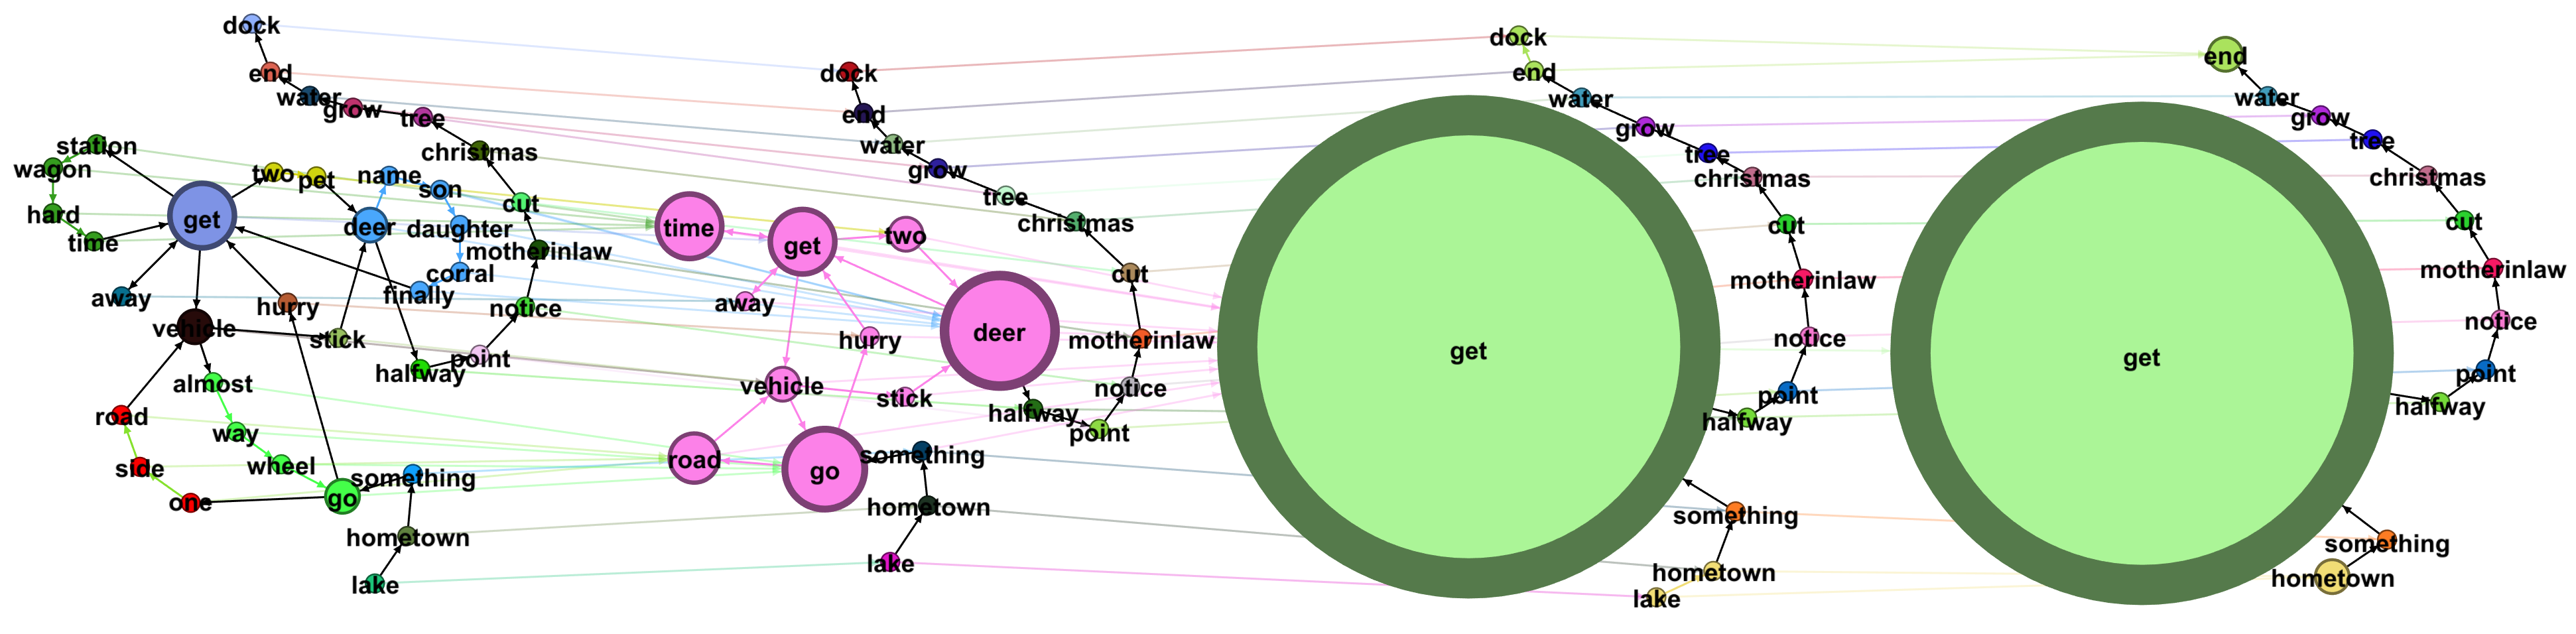
\includegraphics[width=1\textwidth]{Immagini/arlie_dream_graph_example}
    \caption{Grafo multi-livello di un sogno di Arlie}
    \label{fig:arlie-dream-graph}
\end{figure}

In Figura~\ref{fig:arlie-dream-graph} è mostrato un esempio di grafo delle parole costruito a partire da un sogno di Arlie, e dei
relativi livelli di astrazione ottenuti attraverso la contrazione del grafo.
In particolare, l'esempio mostra il grafo multi-livello risultante dall'applicazione di schemi di contrazione per
circuiti semplici, componenti fortemente connesse e stelle.
La funzione di contrazione per stelle rappresenta un ulteriore livello di astrazione, in cui tutti i nodi su cui è
incidente un unico arco che li collega ad un nodo centrale vengono contratti in un unico supernodo.
Nel caso delle parole, il centro di una stella può rappresentante il concetto di base comune a tutti i nodi contratti,
in quanto loro unico punto di collegamento con le altre parole del grafo.

I grafi multi-livello così prodotti sono stati quindi utilizzati come base per l'analisi multi-livello dei sogni,
come descritto nella sezione successiva.

\subsection{Analisi dei risultati}
A partire dall'analisi di un dataset di narrazioni di sogni provenienti da sedici individui si è seguita la
metodologia precedentemente descritta, raccogliendo dati statistici sulle caratteristiche topologiche
dei grafi a vari livelli delle gerarchie prodotte per ciascun sognatore.
In questa parte l'attenzione verrà rivolta a tre particolari sognatori dei sedici originali: Arlie, Emma e Norman.
Arlie è stata identificata come un sognatrice con grafi delle parole aventi parametri strutturali che più si
avvicinano alle medie del campione, mentre Emma e Norman sono stati scelti per alcune caratteristiche atipiche
che li differenziano dal resto del gruppo.

Il grafo multi-livello $M = (G, \Gamma)$ scelto per l'elaborazione del grafo delle parole $G$ prodotto a partire
da ciascun sogno prevede una sequenza di sette funzioni di contrazione che sono, rispettivamente:
\begin{enumerate}[(i)]
    \item \eqmakebox[things][l]{$f_{C_1}$}
    $ \begin{aligned}[t]
      \text{funzione di contrazione per circuiti semplici}
      \end{aligned} $
    \item \eqmakebox[things][l]{$f_{C_2}$}
    $ \begin{aligned}[t]
      \text{funzione di contrazione per componenti fortemente connesse}
      \end{aligned} $
    \item \eqmakebox[things][l]{$f_{C_3},\ldots,f_{C_7}$}
    $ \begin{aligned}[t]
      \text{funzioni di contrazione per stelle}
      \end{aligned} $
\end{enumerate}

Ciascuno dei grafici presentati di seguito comprende tre traiettorie distinte, ognuna corrispondente ai dati
dei tre sognatori selezionati, ottenuti da un insieme di 221, 1252 e 669 narrazioni, rispettivamente.
Per ciascun insieme di narrazioni legate ai particolari sognatori, si sono selezionati i sogni con un numero di
occorrenze di lemmi compreso tra 15 e 300 per narrazione, approssimativamente corrispondenti a sogni
di lunghezze che variano dalle 30 alle 750 parole.
I grafici mostrano l'evoluzione di una certa proprietà dei grafi a ciascun livello della gerarchia,
dove il livello 0 rappresenta la struttura originale del grafo.
L'asse delle ordinate quantifica la proprietà, mentre l'asse delle ascisse delinea i livelli del grafo multi-livello.

A causa della significativa variazione nel numero medio di lemmi tra le narrazioni dei sognatori — per precisione 38,57
per Emma, 28,80 per Norman e 48,47 per Arlie — i dati sensibili alla lunghezza del sogno sono stati normalizzati a un
valore percentuale relativo al conteggio dei lemmi del sogno originale.
A partire da osservazioni effettuate sul dataset, infatti, dati come il numero di nodi e archi, il peso dei nodi,
la dimensione degli insiemi componenti e il numero (ma non la lunghezza) delle basi cicliche risultano essere tutti
linearmente influenzati dal numero di lemmi considerati in ciascun sogno.

Nella Figura~\ref{fig},in alto, è mostrato il grafico del conteggio dei nodi, il quale illustra l'evoluzione della
quantità di nodi nei vari livelli.
I cali significativi delle traiettorie che scendono velocemente a partire da un valore alto indicano una struttura
di nodi inizialmente complessa che subisce una rapida semplificazione.
I dati di Arlie mostrano una una discesa più ripida, suggerendo una veloce contrazione della struttura iniziale sin
dai primi schemi di contrazione.
I dati di Norman e Emma presentano un tasso di declino più contenuto, mantenendo una riduzione coerente rispetto
allo specifico schema di contrazione, indicativo di strutture meno organizzate.

Il grafico del conteggio delle archi imita l'analisi ottenuta dal conteggio dei nodi, fornendo un'idea più chiara
della complessità delle strutture.
Analogamente al conteggio dei nodi, un valore iniziale alto sulle ordinate seguito da un brusco calo suggerisce
una connettività iniziale densa che subisce una significativa semplificazione.
I dati sui sogni di Arlie mostrano una densità di archi ordinaria con un marcato declino al livello 2, indicando una
sostanziale interconnessione di parole.
Essendo che tali interconnessioni derivano da una quantità di archi al livello 1 proporzionalmente
paragonabile a quella degli altri due sognatori, questo aspetto potrebbe suggerire una maggiore qualità delle relazioni
tra le parole nei sogni di Arlie, intesa come una più equa distribuzione degli archi tra parole e cicli di parole.

Il grafico in Figura~\ref{fig} permette di arricchire la visione fornita dai grafici precedenti, mostrando la
percentuale di contrazione dei nodi di ciascun livello, calcolata considerando la quantità di nodi del livello
rispetto a quella del livello precedente.
Le linee indicano che, mentre Emma e Norman presentano solo lievi differenze nelle prime contrazioni per stelle, i dati
di Arlie mostrano una divergenza più significativa nel processo di contrazione delle componenti fortemente connesse.
Questa informazione, combinata con le quelle fornite dai grafici precedenti, suggerisce che molti nodi vengono esclusi
dalle aggregazioni principali, portando a una struttura più frammentata.
Tuttavia, questa struttura si semplifica rapidamente nei livelli successivi, indicando che la maggior parte dei nodi
orbita nelle immediate vicinanze delle massicce aggregazioni principali.

In Figura~\ref{fig} i grafici danno un'idea dell'evoluzione della distribuzione del peso dei nodi.
Al livello iniziale, i dati di Arlie mostrano un peso medio dei nodi moderato, seguito da un marcato aumento nel
corso dei livelli superiori.
Questo modello suggerisce che, mentre le strutture iniziali possiedono nodi di moderata importanza,
l'aggregazione per componenti fortemente connesse amplifica particolarmente la loro rilevanza, risultando in
aggregazioni altamente pesanti.
Ciò non risulta particolarmente evidente nel caso degli altri due sognatori che mantengono un incremento del peso
medio più tendente al rettilineo.
In particolare, i dati di Emma dimostrano un aumento moderato ma costante del peso medio dei nodi, indicativo di
una struttura iniziale equilibrata in cui i nodi acquisiscono gradualmente importanza attraverso i livelli successivi.
D'altra parte, i dati di Norman mostrano un aumento leggermente più pronunciato, a partire dai cicli fino ai
livelli superiori, riflettendo una più bassa dispersione delle singole parole rispetto ad Emma, e una maggiore
inclinazione all'aggregazione, specialmente per le formazioni a stella.
Il grafico della varianza sul peso dei nodi fornisce informazioni sull'equilibrio interno delle strutture rispetto
alla loro importanza.
I dati di Arlie mostrano un forte aumento della varianza, con un picco notevole al livello $2$, indicando una convergenza
di molti nodi verso poche aggregazioni altamente significative ed evidenziando nuovamente l'importanza delle componenti
fortemente connesse nel processo di aggregazione.
I dati di Emma presentano una varianza più alta ai livelli superiori, suggerendo la frequente presenza di nodi
poco pesanti che rimangono distaccati dalle aggregazioni principali e che, quindi, sono generalmente distanti, poco
connessi o situati in fondo a cammini che rappresentano vicoli ciechi.

Il grafico delle medie dei cammino minimi in Figura~\ref{fig} rappresenta l'evoluzione della lunghezza media di tali
cammini attraverso i diversi livelli dei grafi.
Tale misura è calcolata sulla versione non orientata di ciascun grafo come la distanza media tra ciascuna coppia di
nodi in termini di archi.
Valori iniziali più alti indicano strutture iniziali più estese, le quali normalmente riducono tale caratteristica
contraendosi attraverso i livelli successivi.
I dati di Emma iniziano con cammini mediamente lunghi, da cui si deduce la presenza percorsi inizialmente isolati
che diventano via via più compatti rispetto al resto del grafo, specialmente con la contrazione dei cicli.
Tuttavia, i grafi delle parole di Emma dimostrano di mantenere un'elevata lunghezza media, corroborando l'ipotesi
della frequente presenza di lunghi vicoli ciechi.
I dati di Norman mostrano cammini di lunghezze più moderate, imitando l'andamento di Emma,
mentre i dati di Arlie presentano cammini inizialmente più lunghi e con declino più graduale, indicando strutture di
percorso più semplici.
Il secondo grafico nella stessa figura mostra l'evoluzione del diametro del grafo, parametro strettamente legato
alla lunghezza dei cammini minimi, definito come il cammino minimo massimo tra tutte le coppie di nodi.
Diametri iniziali più alti indicano strutture più estese. Questo grafico segue accuratamente quello precedente,
indicando che, per tutti e tre i sognatori, le forme del grafo tra i livelli non sono deformate e contengono nodi
approssimativamente equidistanti.

Il grafico del conteggio delle basi cicliche in Figura~\ref{fig} quantifica la presenza di collegamenti circolari tra
parole o gruppi di parole, considerando la versione non orientata dei grafi.
Le basi cicliche rappresentano i cicli fondamentali del grafo non ulteriormente scomponibili in sotto-cicli.
Sono dette ``basi'' in quanto a partire da esse è possibile comporre tutti gli altri cicli attraverso una operazione di
unione degli archi che li compongono in or esclusivo.
I dati di Norman mostrano un alto conteggio iniziale dei cicli seguiti da un brusco calo, indicando la presenza di molti
cicli orientati tra le basi cicliche che vengono riconosciute nella prima funzione di contrazione.
I dati di Arlie presentano più basi cicliche che non sono facilmente contratte al primo livello di contrazione,
indicando una maggiore presenza di connessioni cicliche nascoste che non seguono un semplice percorso unidirezionale.
I dati di Emma mostrano meno cicli con una diminuzione costante, indicando la presenza di strutture più lineari.
Queste informazioni, combinate ai dati del grafico sulla lunghezza delle basi cicliche, suggeriscono che i sogni di
Norman contengono più cicli, anche se più piccoli, mentre i sogni di Emma contengono una minor quantità di cicli,
seppur generalmente più grandi.
Tuttavia, la distinzione sulla lunghezza tra Emma e Arlie può essere osservata solo nel grafo al livello 1, suggerendo
che, a differenza di Arlie, le basi cicliche di Emma sono ottenute prevalentemente da insiemi di parole che si
conseguono nella narrazione originale del sogno, nonostante consistano di un alto numero di lemmi.

La Figura~\ref{fig} illustra la densità media dei grafi per ciascun livello, dove la densità di un grafo è definita
come il rapporto tra il numero di archi nel grafo e il numero di archi possibili.
Tutti e tre i sognatori iniziano con basse densità iniziali del grafo che aumentano attraverso i primi livelli di
contrazione.
Oltre che essere una naturale conseguenza della riduzione della dimensione del grafo, questo indica che le strutture
iniziali di singole parole sparse diventano più interconnesse quando i nodi rappresentano aggregazioni di parole
correlate.
Le narrazioni di Arlie mostrano l'aumento di densità più elevato nel corso dei primi livelli di contrazione,
suggerendo un'interconnessione più complessa tra le componenti fortemente connesse, che si semplifica
rapidamente nei livelli successivi.
Livelli di densità bassi ai livelli superiori possono anche indicare una maggiore tendenza alla presenza di
un unico grande cluster di parole.
Osservando gli altri due sognatori, è interessante notare che, mentre i sogni di Norman mostrano una densità più alta
rispetto a quelli di Emma nei livelli iniziali, i dati dei due sognatori convergono a valori simili nei livelli
superiori, indicando un livello simile di interconnessione tra le aggregazioni principali.

Il grafico del coefficiente di assortatività dei pesi in Figura~\ref{fig} fornisce informazioni sull'evoluzione
di tale valore tra i singoli nodi.
L'assortatività è un parametro che misura la tendenza dei nodi con determinate caratteristiche numeriche a collegarsi
con nodi aventi caratteristiche simili e, in questo caso, indica la tendenza dei nodi con pesi simili a connettersi tra
loro.
Un coefficiente positivo suggerisce la presenza di una tendenza per i temi predominanti a connettersi direttamente
tra loro, mentre un coefficiente negativo indica una tendenza per i nodi pesanti a connettersi con nodi di peso esiguo.
Questo potrebbe essere particolarmente rilevante nei livelli avanzati, dove i temi principali del sogno sono già ben
definiti.
I sogni di Norman sono soggetti ad un evidente calo dell'assortatività ai livelli alti, indicando, possibilmente,
la presenza ricorrente di una contrazione principale circondata da nodi meno importanti.
I dati di Emma, invece, mostrano una tendenza più stabile, suggerendo che le aggregazioni principali sono tipicamente
interconnesse tra loro e che non possano facilmente essere ridotte a un singolo nodo che rappresenti una formazione a
stella.

\nlparagraph{Confronto con gli studi correlati}

Studi correlati già citati, che riguardano tecniche di analisi dei sogni basate su grafi, hanno osservato differenze
nelle caratteristiche topologiche dei grafi a partire da gruppi di persone pre-classificate come sognatori sani,
schizofrenici o bipolari.
In particolare, i grafi associati ai sogni di pazienti schizofrenici sono stati valutati come grafi generalmente
piccoli e poco connessi, con basso numero di cicli, un elevato diametro rapportato alla dimensione del grafo e un
basso coefficiente di clustering, il quale indica la tendenza dei nodi a formare cluster densamente connessi.
I grafi dei pazienti bipolari, sebbene abbiano dimostrato avere un numero inferiore di caratteristiche che permettono
di distinguerli rispetto al gruppo di controllo, sono prevalentemente caratterizzati da alta connettività, alta densità
e alto coefficiente di clustering, abbinato alla maggiore presenza di cicli brevi e un basso diametro.
Tuttavia la caratteristica che ha permesso di caratterizzare e riconoscere distintamente il gruppo di controllo
dagli altri due è la presenza e la dimensione delle componenti fortemente connesse: i sognatori del controllo hanno
mostrato la dimensione maggiore tra tutti, seguiti dai bipolari e, per ultimi, gli schizofrenici. \newline

Per via del fatto che i dati ottenuti in questa analisi non sono corredati da informazioni riguardanti lo stato di
salute mentale dei sognatori, i risultati sono stati confrontati con quelli degli studi precedenti al fine
di trarre delle ipotesi su una possibile classificazione dei sognatori.
I risultati dell'analisi multi-livello si correlano alle scoperte già consolidate suggerendo che Arlie potrebbe essere
collocata nel gruppo di controllo, a causa dell'alta rilevanza delle componenti fortemente connesse nel processo di
contrazione e di altri parametri riguardanti la connettività e l'alto grado dei nodi.
Questa ipotesi è supportata dal fatto che i grafici di Arlie si conformano ai valori medi dei sedici sognatori nel
dataset.
Al contrario, Emma ha presentato caratteristiche tipiche dei pazienti schizofrenici, come un diametro del grafo
elevato e un basso coefficiente di clustering, indicando nodi poco connessi.
Dai dati di Norman, nel mentre, è emersa una rilevanza dei cicli e un alto coefficiente di clustering, che potrebbero
essere considerate qualità simili ai sogni dei pazienti bipolari.
Si noti, tuttavia, che molti altri sono stati gli aspetti emersi dall'analisi multi-livello, i quali hanno fornito una
visione più completa sui sognatori rispetto a quella che si sarebbe ottenuta da un'analisi a livello singolo.

